% SETUP
\documentclass[11pt]{article}
\linespread{1.1}
\usepackage[utf8]{inputenc}
\usepackage{graphicx, amsmath, array, graphics, amssymb, epsfig, psfrag, geometry, alltt, subfiles, blindtext, pdfpages, mathtools, float}
\usepackage[export]{adjustbox}
\usepackage{fancyhdr}
\usepackage{array}
\usepackage{hyperref}

%%%%%%%%%%%%%%  code listing
\usepackage{listings}
\usepackage{color} %red, green, blue, yellow, cyan, magenta, black, white
\definecolor{mygreen}{RGB}{2,94,33} % color values Red, Green, Blue
\definecolor{mylilas}{RGB}{170,55,241}

\lstset{language=Matlab,%
    %basicstyle=\color{red},
    breaklines=true,%
    morekeywords={matlab2tikz},
    keywordstyle=\color{blue},%
    morekeywords=[2]{1}, keywordstyle=[2]{\color{black}},
    identifierstyle=\color{black},%
    stringstyle=\color{mylilas},
    commentstyle=\color{mygreen},%
    showstringspaces=false,%without this there will be a symbol in the places where there is a space
    numbers=left,%
    numberstyle={\tiny \color{black}},% size of the numbers
    numbersep=9pt, % this defines how far the numbers are from the text
    emph=[1]{for,end,break},emphstyle=[1]\color{black}, %some words to emphasise
    %emph=[2]{word1,word2}, emphstyle=[2]{style},    
}

\geometry{a4paper, top = 20mm, bottom = 20mm, left = 15mm, right = 15mm}
\DeclarePairedDelimiter\set\{\}

% Headers
\pagestyle{fancy}
\fancyhf{}
\chead{ELEN90064 Advanced Control Systems - Workshop 5 Report}
\cfoot{\thepage}

\begin{document}
% Cover Sheet
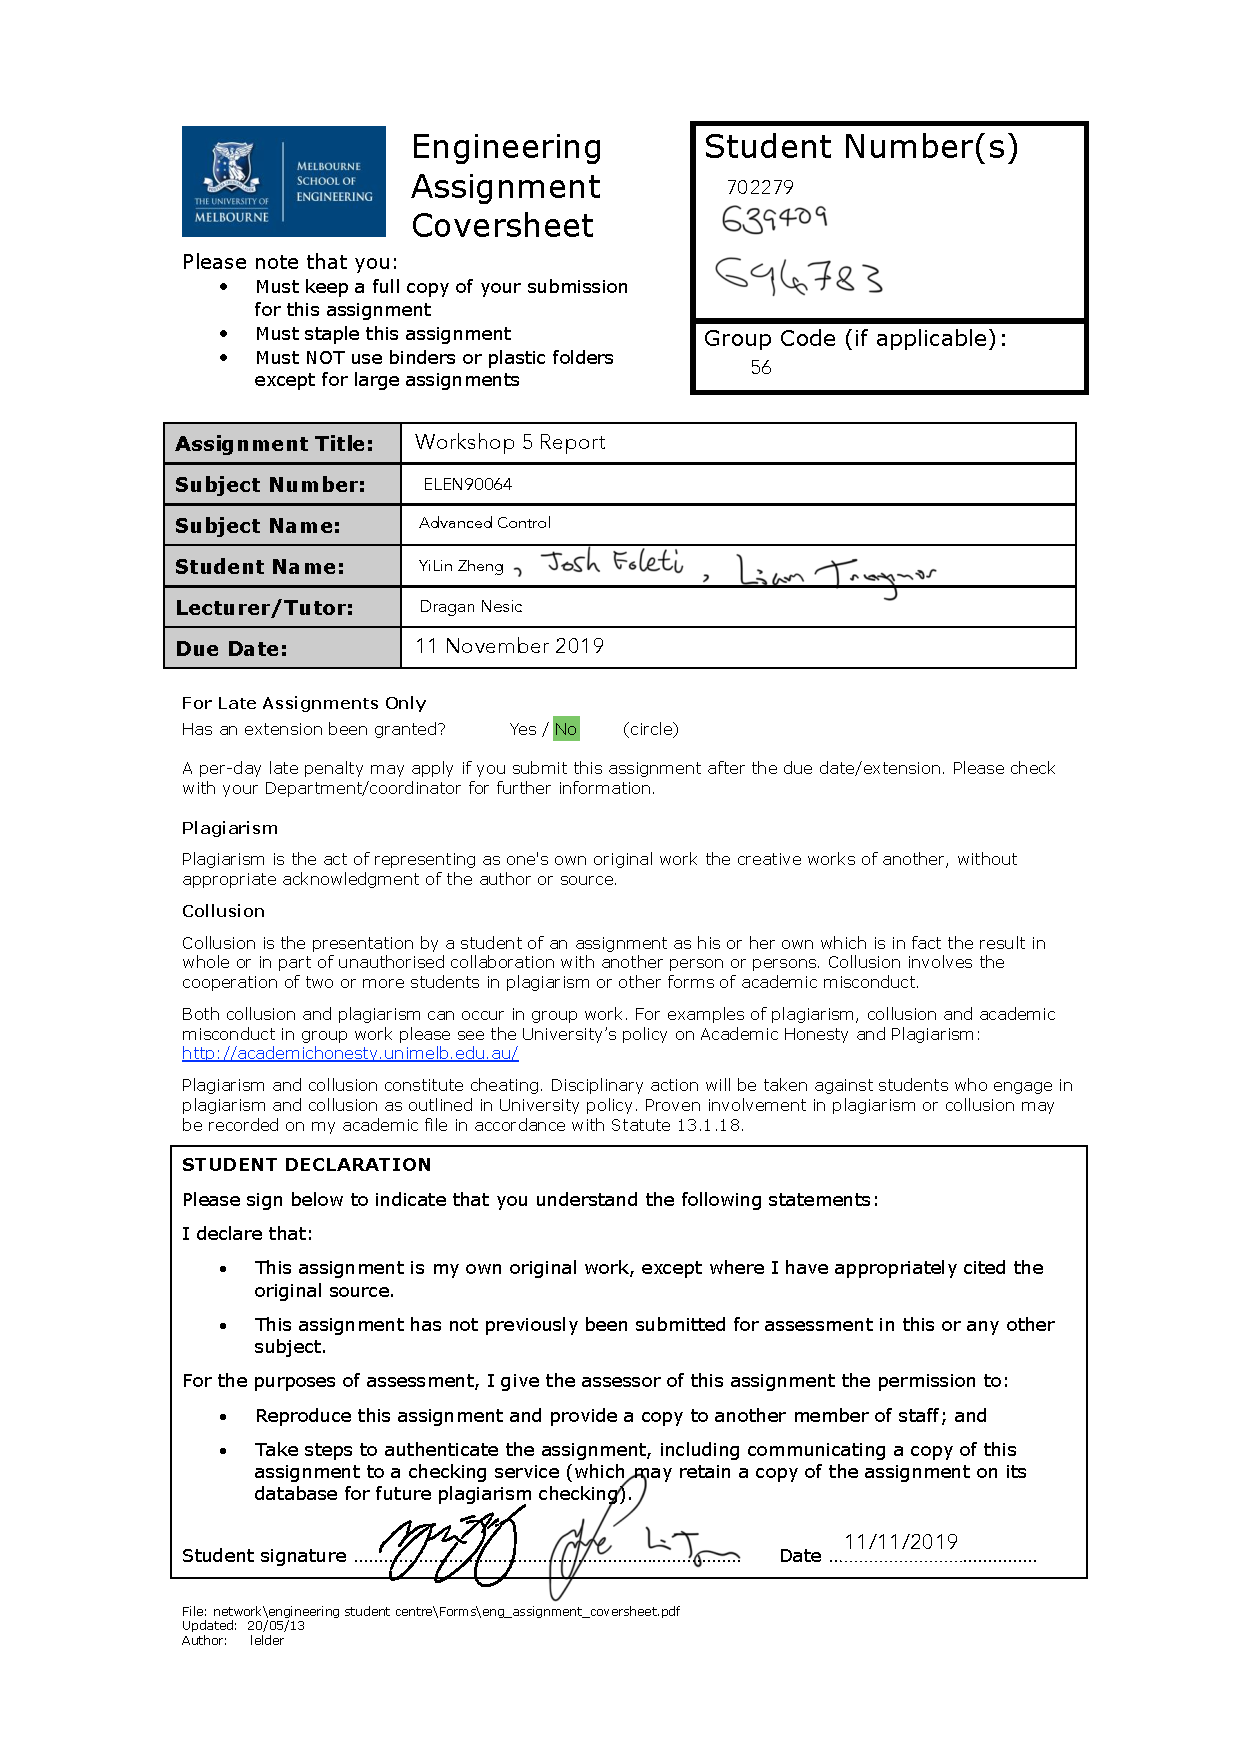
\includepdf{EngCSW5.pdf}
\clearpage
\setcounter{page}{1}

% Title
\begin{center}
\textbf{\Large{Internal Model Principle based LQG Control for 2 DOF Configuration}}\\
Group 56: Josh Foleti [639409], Liam Traynor [694783], YiLin Inez Zheng [702279], \\
Workshop: Friday 1:00pm - 3:00pm Luis, Due: 11/11/19  
\end{center}

%%%%%%%%%%%%% BEGIN INTRODUCTION %%%%%%%%%%%%%%%%%
\section{Introduction}
The main objective in this workshop is to select design parameters that actuate the Quanser Aero.

% Some description about what we did, steps for analysis and design
\subsection{Method}

%%%%%%%%%%%% BEGIN SYSTEM MODELLING SECTION %%%%%%%%%%%%%%%%
\section{System Modelling}
% Calculations and Simulation Results go here

%%%%%%%%%%%% BEGIN IMPLEMENTATION SECTION %%%%%%%%%%%%%%%%
\section{Implementation and Testing}
% Experimental Results and Discussion

%%%%%%%%%%%% BEGIN CONCLUSION %%%%%%%%%%%%%%%%
\section{Conclusions}

\end{document}
